%  LaTeX support: latex@mdpi.com
%  For support, please attach all files needed for compiling as well as the log file, and specify your operating system, LaTeX version, and LaTeX editor.

%=================================================================
\documentclass[algorithms,article,submit,pdftex,moreauthors]{Definitions/mdpi}

%--------------------
% Class Options:
%--------------------
%----------
% journal
%----------
% Choose between the following MDPI journals:
% acoustics, actuators, addictions, admsci, adolescents, aerobiology, aerospace, agriculture, agriengineering, agrochemicals, agronomy, ai, air, algorithms, allergies, alloys, analytica, analytics, anatomia, animals, antibiotics, antibodies, antioxidants, applbiosci, appliedchem, appliedmath, applmech, applmicrobiol, applnano, applsci, aquacj, architecture, arm, arthropoda, arts, asc, asi, astronomy, atmosphere, atoms, audiolres, automation, axioms, bacteria, batteries, bdcc, behavsci, beverages, biochem, bioengineering, biologics, biology, biomass, biomechanics, biomed, biomedicines, biomedinformatics, biomimetics, biomolecules, biophysica, biosensors, biotech, birds, bloods, blsf, brainsci, breath, buildings, businesses, cancers, carbon, cardiogenetics, catalysts, cells, ceramics, challenges, chemengineering, chemistry, chemosensors, chemproc, children, chips, cimb, civileng, cleantechnol, climate, clinpract, clockssleep, cmd, coasts, coatings, colloids, colorants, commodities, compounds, computation, computers, condensedmatter, conservation, constrmater, cosmetics, covid, crops, cryptography, crystals, csmf, ctn, curroncol, cyber, dairy, data, ddc, dentistry, dermato, dermatopathology, designs, devices, diabetology, diagnostics, dietetics, digital, disabilities, diseases, diversity, dna, drones, dynamics, earth, ebj, ecologies, econometrics, economies, education, ejihpe, electricity, electrochem, electronicmat, electronics, encyclopedia, endocrines, energies, eng, engproc, entomology, entropy, environments, environsciproc, epidemiologia, epigenomes, est, fermentation, fibers, fintech, fire, fishes, fluids, foods, forecasting, forensicsci, forests, foundations, fractalfract, fuels, future, futureinternet, futurepharmacol, futurephys, futuretransp, galaxies, games, gases, gastroent, gastrointestdisord, gels, genealogy, genes, geographies, geohazards, geomatics, geosciences, geotechnics, geriatrics, grasses, gucdd, hazardousmatters, healthcare, hearts, hemato, hematolrep, heritage, higheredu, highthroughput, histories, horticulturae, hospitals, humanities, humans, hydrobiology, hydrogen, hydrology, hygiene, idr, ijerph, ijfs, ijgi, ijms, ijns, ijpb, ijtm, ijtpp, ime, immuno, informatics, information, infrastructures, inorganics, insects, instruments, inventions, iot, j, jal, jcdd, jcm, jcp, jcs, jcto, jdb, jeta, jfb, jfmk, jimaging, jintelligence, jlpea, jmmp, jmp, jmse, jne, jnt, jof, joitmc, jor, journalmedia, jox, jpm, jrfm, jsan, jtaer, jvd, jzbg, kidneydial, kinasesphosphatases, knowledge, land, languages, laws, life, liquids, literature, livers, logics, logistics, lubricants, lymphatics, machines, macromol, magnetism, magnetochemistry, make, marinedrugs, materials, materproc, mathematics, mca, measurements, medicina, medicines, medsci, membranes, merits, metabolites, metals, meteorology, methane, metrology, micro, microarrays, microbiolres, micromachines, microorganisms, microplastics, minerals, mining, modelling, molbank, molecules, mps, msf, mti, muscles, nanoenergyadv, nanomanufacturing,\gdef\@continuouspages{yes}} nanomaterials, ncrna, ndt, network, neuroglia, neurolint, neurosci, nitrogen, notspecified, %%nri, nursrep, nutraceuticals, nutrients, obesities, oceans, ohbm, onco, %oncopathology, optics, oral, organics, organoids, osteology, oxygen, parasites, parasitologia, particles, pathogens, pathophysiology, pediatrrep, pharmaceuticals, pharmaceutics, pharmacoepidemiology,\gdef\@ISSN{2813-0618}\gdef\@continuous pharmacy, philosophies, photochem, photonics, phycology, physchem, physics, physiologia, plants, plasma, platforms, pollutants, polymers, polysaccharides, poultry, powders, preprints, proceedings, processes, prosthesis, proteomes, psf, psych, psychiatryint, psychoactives, publications, quantumrep, quaternary, qubs, radiation, reactions, receptors, recycling, regeneration, religions, remotesensing, reports, reprodmed, resources, rheumato, risks, robotics, ruminants, safety, sci, scipharm, sclerosis, seeds, sensors, separations, sexes, signals, sinusitis, skins, smartcities, sna, societies, socsci, software, soilsystems, solar, solids, spectroscj, sports, standards, stats, std, stresses, surfaces, surgeries, suschem, sustainability, symmetry, synbio, systems, targets, taxonomy, technologies, telecom, test, textiles, thalassrep, thermo, tomography, tourismhosp, toxics, toxins, transplantology, transportation, traumacare, traumas, tropicalmed, universe, urbansci, uro, vaccines, vehicles, venereology, vetsci, vibration, virtualworlds, viruses, vision, waste, water, wem, wevj, wind, women, world, youth, zoonoticdis
% For posting an early version of this manuscript as a preprint, you may use "preprints" as the journal. Changing "submit" to "accept" before posting will remove line numbers.

%---------
% article
%---------
% The default type of manuscript is "article", but can be replaced by:
% abstract, addendum, article, book, bookreview, briefreport, casereport, comment, commentary, communication, conferenceproceedings, correction, conferencereport, entry, expressionofconcern, extendedabstract, datadescriptor, editorial, essay, erratum, hypothesis, interestingimage, obituary, opinion, projectreport, reply, retraction, review, perspective, protocol, shortnote, studyprotocol, systematicreview, supfile, technicalnote, viewpoint, guidelines, registeredreport, tutorial
% supfile = supplementary materials

%----------
% submit
%----------
% The class option "submit" will be changed to "accept" by the Editorial Office when the paper is accepted. This will only make changes to the frontpage (e.g., the logo of the journal will get visible), the headings, and the copyright information. Also, line numbering will be removed. Journal info and pagination for accepted papers will also be assigned by the Editorial Office.

%------------------
% moreauthors
%------------------
% If there is only one author the class option oneauthor should be used. Otherwise use the class option moreauthors.

%---------
% pdftex
%---------
% The option pdftex is for use with pdfLaTeX. Remove "pdftex" for (1) compiling with LaTeX & dvi2pdf (if eps figures are used) or for (2) compiling with XeLaTeX.

%=================================================================
% MDPI internal commands - do not modify
\firstpage{1}
\makeatletter
\setcounter{page}{\@firstpage}
\makeatother
\pubvolume{1}
\issuenum{1}
\articlenumber{0}
\pubyear{2023}
\copyrightyear{2023}
%\externaleditor{Academic Editor: Firstname Lastname}
\datereceived{ }
\daterevised{ } % Comment out if no revised date
\dateaccepted{ }
\datepublished{ }
%\datecorrected{} % For corrected papers: "Corrected: XXX" date in the original paper.
%\dateretracted{} % For corrected papers: "Retracted: XXX" date in the original paper.
\hreflink{https://doi.org/} % If needed use \linebreak
%\doinum{}
%\pdfoutput=1 % Uncommented for upload to arXiv.org

%=================================================================
% Add packages and commands here. The following packages are loaded in our class file: fontenc, inputenc, calc, indentfirst, fancyhdr, graphicx, epstopdf, lastpage, ifthen, float, amsmath, amssymb, lineno, setspace, enumitem, mathpazo, booktabs, titlesec, etoolbox, tabto, xcolor, colortbl, soul, multirow, microtype, tikz, totcount, changepage, attrib, upgreek, array, tabularx, pbox, ragged2e, tocloft, marginnote, marginfix, enotez, amsthm, natbib, hyperref, cleveref, scrextend, url, geometry, newfloat, caption, draftwatermark, seqsplit
% cleveref: load \crefname definitions after \begin{document}

\usepackage{gensymb}
\usepackage{accents}
\usepackage{xspace}
\usepackage[labelformat=simple]{subcaption}
\renewcommand\thesubfigure{\alph{subfigure}}
\DeclareCaptionLabelFormat{subcaptionlabel}{\normalfont(\textbf{#2}\normalfont)}
\captionsetup[subfigure]{labelformat=subcaptionlabel}

\DeclareRobustCommand{\w}{\mbox{\large\ensuremath{\mathsf{w}}}}
\DeclareRobustCommand{\dotp}{\boldsymbol{\cdot}}
\DeclareRobustCommand{\e}[1]{{\rm e}^{#1}}
%\DeclareRobustCommand{\lay}[1]{^{(#1)}}
\DeclareRobustCommand{\lay}[1]{_{[#1]}}
\DeclareRobustCommand{\mdot}[1]{\accentset{\mbox{\bfseries .}}{#1}}
\DeclareRobustCommand{\ie}{i.e.,\@\xspace}
\DeclareRobustCommand{\eal}{et al.\@\xspace}
\DeclareRobustCommand{\eg}{e.g.,\@\xspace}
\DeclareRobustCommand{\RMSE}{\text{E}_\text{RMS}}
\DeclareRobustCommand{\MARE}{\text{E}_\text{MAR}}
\DeclareRobustCommand{\R}{\text{R}}
\DeclareRobustCommand{\ps}{\text{s}^{-1}}
\DeclareRobustCommand{\mr}[2]{\multirow{#1}{*}{#2}}
\DeclareRobustCommand{\MPa}{\text{MPa}}
\DeclareRobustCommand{\ccirc}{\kern0.5ex\vcenter{\hbox{$\scriptstyle\circ$}}\kern0.5ex}

% This is used to add comments into the text
%
% Will have to be removed from final version
%
\usepackage{soul}
\usepackage{color}
\definecolor{VWyellow}{RGB}{255,251,150}
\DeclareRobustCommand{\OP}[1]{\begingroup\sethlcolor{VWyellow}\textcolor{red}{\hl{\textbf{O.P.:} #1}}\endgroup}
\DeclareRobustCommand{\OPP}[1]{\begingroup\sethlcolor{VWyellow}\textcolor{red}{\hl{\textbf{O.P.:} In previous sentence #1}}\endgroup}

%=================================================================
% Please use the following mathematics environments: Theorem, Lemma, Corollary, Proposition, Characterization, Property, Problem, Example, ExamplesandDefinitions, Hypothesis, Remark, Definition, Notation, Assumption
%% For proofs, please use the proof environment (the amsthm package is loaded by the MDPI class).

%=================================================================
% Full title of the paper (Capitalized)
\Title{Title}

% MDPI internal command: Title for citation in the left column
\TitleCitation{Title}

% Author Orchid ID: enter ID or remove command
\newcommand{\orcidauthorA}{0000-0001-7367-5453} % Add \orcidA{} behind the author's name
%\newcommand{\orcidauthorB}{0000-0000-0000-000X} % Add \orcidB{} behind the author's name

% Authors, for the paper (add full first names)
\Author{Olivier Pantal\'{e}\orcidA{}}

%\longauthorlist{yes}

% MDPI internal command: Authors, for metadata in PDF
\AuthorNames{Olivier Pantal\'{e}}

% MDPI internal command: Authors, for citation in the left column
\AuthorCitation{Pantal\'{e}, O.}
% If this is a Chicago style journal: Lastname, Firstname, Firstname Lastname, and Firstname Lastname.

% Affiliations / Addresses (Add [XX] after \address if there is only one affiliation.)
\address[1]{Laboratoire Génie de Production, Institut National Polytechnique/Ecole Nationale d'Ingénieurs de Tarbes, Université de Toulouse, 47 Av d'Azereix, F-65016 Tarbes, France; Olivier.Pantale@enit.fr; Tel.: +33-562442933}

% Current address and/or shared authorship
%\firstnote{Current address: Affiliation 3.}
%\secondnote{These authors contributed equally to this work.}
% The commands \thirdnote{} till \eighthnote{} are available for further notes

%\simplesumm{} % Simple summary

%\conference{} % An extended version of a conference paper

% Abstract (Do not insert blank lines, i.e. \\)
\abstract{A single paragraph of about 200 words maximum. For research articles, abstracts should give a pertinent overview of the work. We strongly encourage authors to use the following style of structured abstracts, but without headings: (1) Background: place the question addressed in a broad context and highlight the purpose of the study; (2) Methods: describe briefly the main methods or treatments applied; (3) Results: summarize the article's main findings; (4) Conclusions: indicate the main conclusions or interpretations. The abstract should be an objective representation of the article, it must not contain results which are not presented and substantiated in the main text and should not exaggerate the main conclusions.}

% Keywords
\keyword{ANN flow law; Constitutive Behavior; Numerical Implementation; VUHARD ; Activation Functions; Abaqus Explicit}

% The fields PACS, MSC, and JEL may be left empty or commented out if not applicable
%\PACS{J0101}
%\MSC{}
%\JEL{}

%%%%%%%%%%%%%%%%%%%%%%%%%%%%%%%%%%%%%%%%%%
% Only for the journal Diversity
%\LSID{\url{http://}}

%%%%%%%%%%%%%%%%%%%%%%%%%%%%%%%%%%%%%%%%%%
% Only for the journal Applied Sciences
%\featuredapplication{Authors are encouraged to provide a concise description of the specific application or a potential application of the work. This section is not mandatory.}
%%%%%%%%%%%%%%%%%%%%%%%%%%%%%%%%%%%%%%%%%%

%%%%%%%%%%%%%%%%%%%%%%%%%%%%%%%%%%%%%%%%%%
% Only for the journal Data
%\dataset{DOI number or link to the deposited data set if the data set is published separately. If the data set shall be published as a supplement to this paper, this field will be filled by the journal editors. In this case, please submit the data set as a supplement.}
%\datasetlicense{License under which the data set is made available (CC0, CC-BY, CC-BY-SA, CC-BY-NC, etc.)}

%%%%%%%%%%%%%%%%%%%%%%%%%%%%%%%%%%%%%%%%%%
% Only for the journal Toxins
%\keycontribution{The breakthroughs or highlights of the manuscript. Authors can write one or two sentences to describe the most important part of the paper.}

%%%%%%%%%%%%%%%%%%%%%%%%%%%%%%%%%%%%%%%%%%
% Only for the journal Encyclopedia
%\encyclopediadef{For entry manuscripts only: please provide a brief overview of the entry title instead of an abstract.}

%%%%%%%%%%%%%%%%%%%%%%%%%%%%%%%%%%%%%%%%%%
% Only for the journal Advances in Respiratory Medicine
%\addhighlights{yes}
%\renewcommand{\addhighlights}{%

%\noindent This is an obligatory section in “Advances in Respiratory Medicine”, whose goal is to increase the discoverability and readability of the article via search engines and other scholars. Highlights should not be a copy of the abstract, but a simple text allowing the reader to quickly and simplified find out what the article is about and what can be cited from it. Each of these parts should be devoted up to 2~bullet points.\vspace{3pt}\\
%\textbf{What are the main findings?}
% \begin{itemize}[labelsep=2.5mm,topsep=-3pt]
% \item First bullet.
% \item Second bullet.
% \end{itemize}\vspace{3pt}
%\textbf{What is the implication of the main finding?}
% \begin{itemize}[labelsep=2.5mm,topsep=-3pt]
% \item First bullet.
% \item Second bullet.
% \end{itemize}
%}

%%%%%%%%%%%%%%%%%%%%%%%%%%%%%%%%%%%%%%%%%%
\begin{document}

%----------------------------------------------------------------------------------
\section{Introduction}\label{sec:Introduction}
%----------------------------------------------------------------------------------

\subsection{Experimental tests and data}
The experimental tests used for this work are identical to those previously published by Tize Mha \eal \cite{Tize-2023-IEP} and concern compression tests on a Gleeble-3800 device of a 3CrMo2 steel.
Only the most relevant information about those experiments is reported here after.
In order to have a more complete knowledge about the compression tests conducted during this study, the interested reader can refer to \cite{Tize-2023-IEP}.

To build the experimental database, 30 compression tests were conducted for 5 temperature levels $1050\celsius$ to $1250\celsius$ and 6 different strain rates $0.001~\ps$ to $5~\ps$.
All strain/stress data is composed of 701 equidistant strain values from $\varepsilon=0.0$ to $\varepsilon=0.7$ in $0.001$ increments.

%----------------------------------------------------------------------------------
\section{Artificial Neural Network flow law}\label{sec:ANN}
%----------------------------------------------------------------------------------
As already proposed in Pantalé \eal \cite{Pantale-2021-EIN, Pantale-2023-DIA}, the approach used here is to implement the constitutive flow law defined by a trained ANN as a Fortran 77 subroutine into the Abaqus finite element code. 
The ANN is trained on the basis of the Gleeble experiments as already introduced in section \ref{sec:Introduction} and is used to compute the value of the flow stress $\sigma$ as a function of the strain $\varepsilon$, the strain rate $\mdot{\varepsilon}$ and the temperature $T$.
After the training phase, the weights and biases of the ANN are transcoded into a Fortran 77 subroutine wich is compiled and linked with lthe libraries of the Abaqus FE code to include the thermomechanical behavior and compute the flow tress and its three derivatives $\partial\sigma/\partial\varepsilon$, $\partial\sigma/\partial\mdot{\varepsilon}$ and $\partial\sigma/\partial T$ needed by the radial-return algorithm of the FE code.

\subsection{ANN governing equations}\label{subsec:ANN-eqn}

\subsubsection{Network architecture}\label{subsubsec:ANN-arch}
According to Figure \ref{fig:ANN-2HL}, the Artificial Neural Network used for computing the flow stress $\sigma$ from the strain $\varepsilon$, the strain rate $\mdot{\varepsilon}$ and the temperature $T$ is a two hidden layers network as already proposed by Pantalé \eal \cite{Pantale-2021-EIN, Pantale-2023-DIA}.
\begin{figure}[h]
\centering
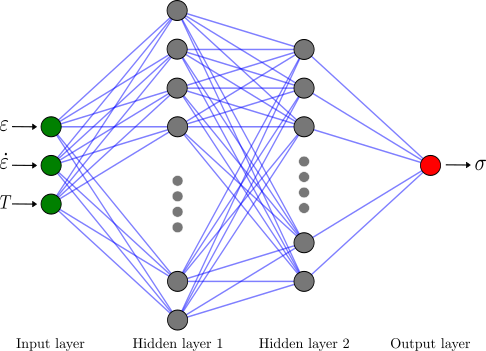
\includegraphics[width=0.55\columnwidth]{Figures/ANN-2HL}
\caption{Two hidden layers artificial neural network architecture with 3 inputs neurons ($\varepsilon$, $\mdot{\varepsilon}$ and $T$) and 1 output neuron ($\sigma$).}
\label{fig:ANN-2HL}
\end{figure}
Conforming to the structure presented in Figure \ref{fig:ANN-2HL}, the input of the neural network is a three component vector noted $\overrightarrow{x}$.

Any hidden layer ($k$), containing $n$ neurons, takes a weighted sum of the outputs $\overrightarrow{\hat{y}}\lay{k-1}$ of the previous layer $(k-1)$, containing $m$ neurons, given by the following equation:
\begin{equation}
\overrightarrow{y}\lay{k} = \w\lay{k} \overrightarrow{\hat{y}}\lay{k-1}+ \overrightarrow{b}\lay{k}\label{eq:ANN-y},
\end{equation}
where $\overrightarrow{y}\lay{k}$ contains the internal values of the neurons from summation at the layer level ($k$), $\w\lay{k}$ is the weight parameter matrix $[n\times m]$ between layer ($k$) and layer $(k-1)$, $\overrightarrow{b}\lay{k}$ is the bias vector of the layer ($k$) and $\overrightarrow{\hat{y}}\lay{k-1}$ is the output vector of the layer $(k-1)$ after the application of the activation function defined here-after.
The total number of learning parameters $N$ for any hidden layer ($k$) is the sum of the number of weights and the number of biases in the layer ($k$), i.e. $N=n(m+1)$.
After the summation operation defined by equation (\ref{eq:ANN-y}), each hidden layer ($k$) provides an output vector $\overrightarrow{\hat{y}\lay{k}}$ calculated from an activation function $f\lay{k}$ according to the following equation:
\begin{equation}
\overrightarrow{\hat{y}}\lay{k}=f\lay{k}(\overrightarrow{y}\lay{k}).
\label{eq:ANN-f}
\end{equation}
This process is repeated for each hidden layer of the neural network until we reach the output layer where the formulation differ, so that the output $s$ of the neural network is given by:
\begin{equation}
s = \overrightarrow{w}^T \dotp \overrightarrow{\hat{y}}\lay{2} + b\label{eq:ANN-s},
\end{equation}
where $\overrightarrow{w}$ is the vector of the output weights of the ANN and $b$ is the bias associated to the output neuron.
As usually done in a regression approach, there is no activation function associated to the output neuron of the network (or some authors consider here a linear activation function).

\subsubsection{Activation functions}\label{subsubsec:ANN-act}

At the heart of ANNs lies the concept of activation functions, pivotal elements that determine how information is transformed within the network's neurons.
The choice of activation functions is a critical design decision, as these functions greatly influence the network's capacity to learn and represent complex patterns in data.
The selection of activation functions is guided by their distinct properties, including non-linearity, differentiability, and computational efficiency.

%An activation function is a function that acts on the output of all neurons of the hidden layers and helps the ANN to learn complex non-linear features of the data to process.
In regression ANNs, the choice of activation functions is typically driven by the need to approximate continuous output values rather than class labels.
Many studies have been proposed concerning the right activation function to use depending on the physical problem to solve such as the review proposed by Dubey \eal \cite{Dubey-2022-AFD} or Jagtap \eal \cite{Jagtap-2023-HIA}.
The key aspect of the activation function is its capacity to introduce non-linearity into the network to capture non-linear features.
Without this non-linearity, the neural network behaves like a linear regression model.
According to and Hornik \eal \cite{Hornik-1989-MFN}, the activation function must be bounded, non-constant, monotonically increasing, and continuous to ensure the universal approximation property of the neural network.
A number of activations functions can be used in neural networks.
They are used to introducing non-linearity in the system of equations.
In a previous published work, we have used mostly the Sigmoid activations function for the ANN flow laws.
In the present paper, we are going to explore other activations functions and their influence on the final results, up-to the implementation into a finite element code such as the Abaqus software.
Among the number of activations functions available in the literature, we have selected the six ones reported in Figure \ref{fig:Act}.
\begin{figure}[h]
\centering
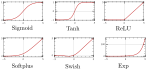
\includegraphics[width=0.8\columnwidth]{Figures/act}
\caption{Activation functions used in artificial neural networks.}
\label{fig:Act}
\end{figure}

The Sigmoid activation function \cite{Han-1995-ISF}, also known as the logistic activation function, is a widely used activation function in artificial neural networks. 
It was originally developed in the field of logistic regression and later adapted for use in neural networks. 
It maps any input to an output in the range $[0,1]$, making it suitable for tasks where the network's output needs to represent probabilities or values between 0 and 1.
The Sigmoid  activation function $f(x)$ and its derivative $f'(x)$ are defined by the following equations:
\begin{equation}
f(x) = \frac{1}{1+\e{-x}}\qquad \text{and}\qquad f'(x) = f(x)\left(1-f(x)\right).\label{eq:act-sig}
\end{equation}
This activation function has been widely used until the early 1990s.
Its main advantage is that it is bounded, while its main drawbacks are the vanishing gradient problem, an output not centered on zero and saturation for large input values.

From 1990s to 2000s, the hyperbolic tangent activation function has been widely used and was preferred for the training of neural networks with respect to the Sigmoid function.
The  hyperbolic tangent function squashes the output within the range $[-1,+1]$ and its formulation is given by the following equations:
\begin{equation}
f(x) = \frac{\e{x} - \e{-x}}{\e{x} + \e{-x}}\qquad \text{and}\qquad f'(x) = 1 - f(x)^2.\label{eq:act-tanh}
\end{equation}
This function is useful when the network needs to model data with mean-centered features, as it can capture both positive and negative correlations.
The Tanh activation function and the Sigmoid activation function are closely related in the sense that they both introduce non-linearity and squash their inputs into bounded ranges.
The evaluation of this activation function requires more CPU time than the Sigmoid function since we need to compute two exponential functions to evaluate $f(x)$.

ReLU is a widely used activation function in classification ANNs due to its simplicity and computational efficiency, as it involves simple thresholding. It introduces non-linearity and is computationally efficient. It outputs the input if it's positive and zero if it's negative:
\begin{equation}
f(x) = \max(0,x)\qquad \text{and}\qquad f'(x) =
\begin{cases}
1&x>0\\
0&x\le 0
\end{cases}.\label{eq:act-relu}
\end{equation}
ReLU mitigates the vanishing gradient problem better than Sigmoid and Tanh, making it suitable for deep networks.
It often leads to faster convergence in training deep neural networks.
The downside of ReLU is with the vanishing gradient problem for all negative inputs.

The Softplus function \cite{Dugas-2000-ISO} approximates the ReLU activation function smoothly. It is defined as the primitive of the Sigmoid function and is written:
\begin{equation}
f(x) = \log\left(1+\e{x}\right)\qquad \text{and}\qquad f'(x) = \frac{1}{1+\e{-x}}.\label{eq:act-softplus}
\end{equation}
Softplus activation function enhances a more gradual transition from zero than ReLU, and can model positive and negative values.
The main drawback is that its computational efficiency is low.

Swish \cite{Ramachandran-2018-SAF} is a smooth and differentiable activation function defined as:
\begin{equation}
f(x) = \frac{x}{1+\e{-x}}\qquad \text{and}\qquad f'(x) =  f(x) + \frac{1 - f(x)}{1+\e{-x}}.\label{eq:act-swish}
\end{equation}
Swish has shown improved performance in some network architectures, especially when used as an activation function in deep learning models.
The simplicity of Swish and its similarity to ReLU make it easy for practitioners to replace ReLUs with Swish units in any neural network.
 
Looking at the shape of the ReLU and Swish functions, apart from those classic activations functions already widely used in ANNs, we propose here-after to add an extra one, based on the exponential function and simply defined by:
\begin{equation}
f(x) = \e{x}\qquad \text{and}\qquad f'(x) = f(x).\label{eq:act-exp}
\end{equation}
The idea here is to use the property so that the derivative of the activation function is defined only by the activation function itself, as well as for the Sigmoid and Tanh, but with the simplest formulation.
This will reduce the CPU cost since we need to compute both the function and its derivative for our implementation in the FE code into a very CPU intensive subroutine

In order to compare the different activation functions, all six activations functions will be used in the rest of this paper and results will be compared in terms of efficiency, and precision of the models.

\subsubsection{Pre and post processing architecture}\label{subsubsec:ANN-pre}
As we are using activations functions enhancing vanishing gradients for large values, the three inputs as well as the output must be normalized within the range $[0,1]$ to avoid ill-conditioning of the neural network.
This range has been chosen because we will use the Sigmoid activation function as one of the six proposed formulations, while this later squashed the output to the lowest range $[0,1]$.

Concerning the inputs, the range and mean values of the input quantities are very different according to the data presented in section \ref{sec:Introduction}.
In our case, the amplitude $\Delta\varepsilon$ and mean value $\overline\varepsilon$ of the strain are $\Delta\varepsilon=0.7$ and $\overline\varepsilon=0.35$ respectively.
Concerning the strain rate $\Delta\mdot{\varepsilon}=4.999~\ps$ and $\overline{\mdot{\varepsilon}}=2.5005~\ps$ and concerning the temperature $\Delta T=200~\celsius$ and $\overline T=1150~\celsius$.

As proposed in Pantalé \eal \cite{Pantale-2021-EIN}, we first substitute  $\ln(\mdot{\varepsilon}/\mdot{\varepsilon}_0)$, with $\mdot{\varepsilon}_0$ equal to the lowest strain rate, for the value of $\mdot{\varepsilon}$.
Then in a second time, we squash the strain, strain rate and temperature within the range $[0,1]$.
Therefore, the three components of the input vector $\overrightarrow{x}$ are calculated from the strain $\varepsilon$, the strain rate $\mdot{\varepsilon}$ and the temperature $T$ using the following expressions:
\begin{equation}
\overrightarrow{x}=
\begin{cases}
x_1 = \dfrac{\varepsilon - [\varepsilon]_{min}}{[\varepsilon]_{max} - [\varepsilon]_{min}}\\
x_2 = \dfrac{\ln(\mdot{\varepsilon}/\mdot{\varepsilon}_0)-[\ln(\mdot{\varepsilon}/\mdot{\varepsilon}_0)]_{min}}{[\ln(\mdot{\varepsilon}/\mdot{\varepsilon}_0)]_{max}-[\ln(\mdot{\varepsilon}/\mdot{\varepsilon}_0)]_{min}}\\
x_3 = \dfrac{T-[T]_{min}}{[T]_{max}-[T]_{min}}
\end{cases},
\label{eq:ANN-input}
\end{equation}
where $[~]_{min}$ and $[~]_{max}$  are the maximum and minimum values of the corresponding field.

The output of the model, \ie the flow stress, enhances the same behavior with $\Delta\sigma=153.7~\MPa$ and $\overline\sigma=63.6~\MPa$. Therefore, we apply the same procedure as previously presented and the flow stress $\sigma$ is related to the output $s$ of the ANN according to the following relation:
\begin{equation}
\sigma =  \left([\sigma]_{max}-[\sigma]_{min}\right)s + [\sigma]_{min}.\label{eq:ANN-output}
\end{equation}

\subsubsection{Derivatives of the Neural Network}\label{subsubsec:ANN-der}

As introduced earlier, in order to implement the ANN as a Fortran 77 subroutine in the Abaqus FE code, we need to compute the three derivatives of the flow stress $\sigma$ with respect to the strain $\varepsilon$, the strain rate $\mdot{\varepsilon}$ and the temperature $T$.

As the network architecture is fixed and known concerning the number of hidden layers, we can compute the derivatives by differentiation the output of the network with respect to the inputs.
As illustrated in Figure \ref{fig:ANN-2HL}, we are concerned here by a two hidden layers neural network. Therefore, as Equations (\ref{eq:ANN-y}-\ref{eq:ANN-s}) are used to compute  $\overrightarrow{y}\lay{k}$ and $\overrightarrow{\hat{y}}\lay{k}$ for each hidden layer and the output $s$ from the input vector $\overrightarrow{x}$ of the ANN we can write the derivative $\overrightarrow{s}'$ of a two hidden layers network as follow:
\begin{equation}
\overrightarrow{s}' = \w\lay{1}^T \dotp\left[\left(\w\lay{2}^T \dotp \left(\overrightarrow{w}^T \ccirc f'(\overrightarrow{y}\lay{2})\right)\right) \ccirc f'(\overrightarrow{y}\lay{1})\right] \label{eq:ANN-der},
\end{equation}
where $f'\left(\square\right)$ is the derivative of the activation function defined by Equations (\ref{eq:act-sig}-\ref{eq:act-exp}) and $\ccirc$ is the Hadamard product (also known as the element-wise product).
Because of the pre and post processing of the values introduced in section \ref{subsubsec:ANN-pre}, the derivative of the flow stress $\sigma$ with respect to the inputs $\varepsilon$, $\mdot{\varepsilon}$ and $T$ is then given by:
\begin{equation}
\begin{cases}
\partial \sigma/\partial \varepsilon = s'_1 \dfrac{[\sigma]_{max} -[\sigma]_{min}}{[\varepsilon]_{max} -[\varepsilon]_{min}}\\
\partial \sigma/\partial\mdot{\varepsilon} = \dfrac{s'_2}{\mdot{\varepsilon}} \dfrac{[\sigma]_{max} -[\sigma]_{min}}{[\mdot{\varepsilon}]_{max} -[\mdot{\varepsilon}]_{min}} \\
\partial \sigma/\partial T = s'_3 \dfrac{[\sigma]_{max} -[\sigma]_{min}}{[T]_{max} -[T]_{min}}
\end{cases}
\label{eq:ANN-der2},
\end{equation}
where $s'_i$ is one of the three components of the vector $\overrightarrow{s}'$ defined by Equation (\ref{eq:ANN-der}).

Finally, Equations (\ref{eq:ANN-y}-\ref{eq:ANN-s}), (\ref{eq:ANN-input}-\ref{eq:ANN-der2}) and the requested activation function defined by one of the Equations (\ref{eq:act-sig}-\ref{eq:act-exp}) will be used to implement the ANN as a Fortran 77 subroutine for the Abaqus FE software as it will be presented in Section \ref{subsec:Num-impl}.

\subsection{Training of the ANN on experimental data}\label{subsec:train}

The Python program used for training the neural network was created with the dedicated Python library, Tensorflow \cite{Tensorflow-2015}.
The training phase employed the Adaptive Moment Estimation (ADAM) optimizer \cite{Kingma-2015-AMS}.
With regard to our previous publications about ANN constitutive flow law \cite{Pantale-2021-EIN}, we have made the choice to use a two hidden layers ANN with 17 neurons for the first hidden layer and 9 neurons for the second hidden layer. 
There is a total number of $240$ trainable parameters to optimize.
As we have 3 inputs and 1 output, we reference each of the ANNs using the notation 3-17-9-1-act, where act refers the activation function used for the model.
All six models have been trained in simultaneously for the same number of iterations ($30~000$ iterations, lasting around 5 hours) on a PowerEdge R730 server running Ubuntu 22.04 LTS 64 bits, 96 GB of Ram, with 2 Intel Xeon CPU E5-2650 2.20GHz.

%\subsubsection{Activation functions analysis\label{subsubsec:ANN-actanal}}

\begin{figure}[h]
\centering
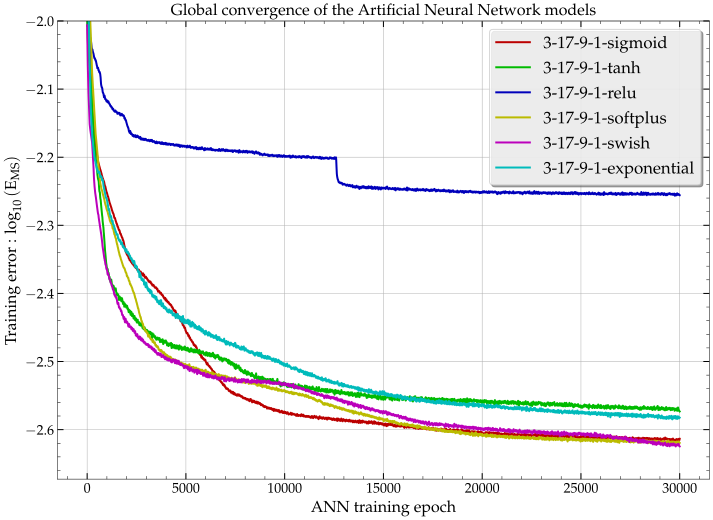
\includegraphics[width=0.8\columnwidth]{Figures/3Cr2Mo-convergence-17-9}
\caption{Global convergence of the six ANN models.}
\label{fig:ANN-conv}
\end{figure}

Figure \ref{fig:ANNFit} shows a comparison of the experimental flow stress measures during the Gleeble compression tests and the predicted flow stress $\sigma$ using the ANN for the strain rate $\mdot{\varepsilon}=1~\ps$. 
\begin{figure}[h]
\centering
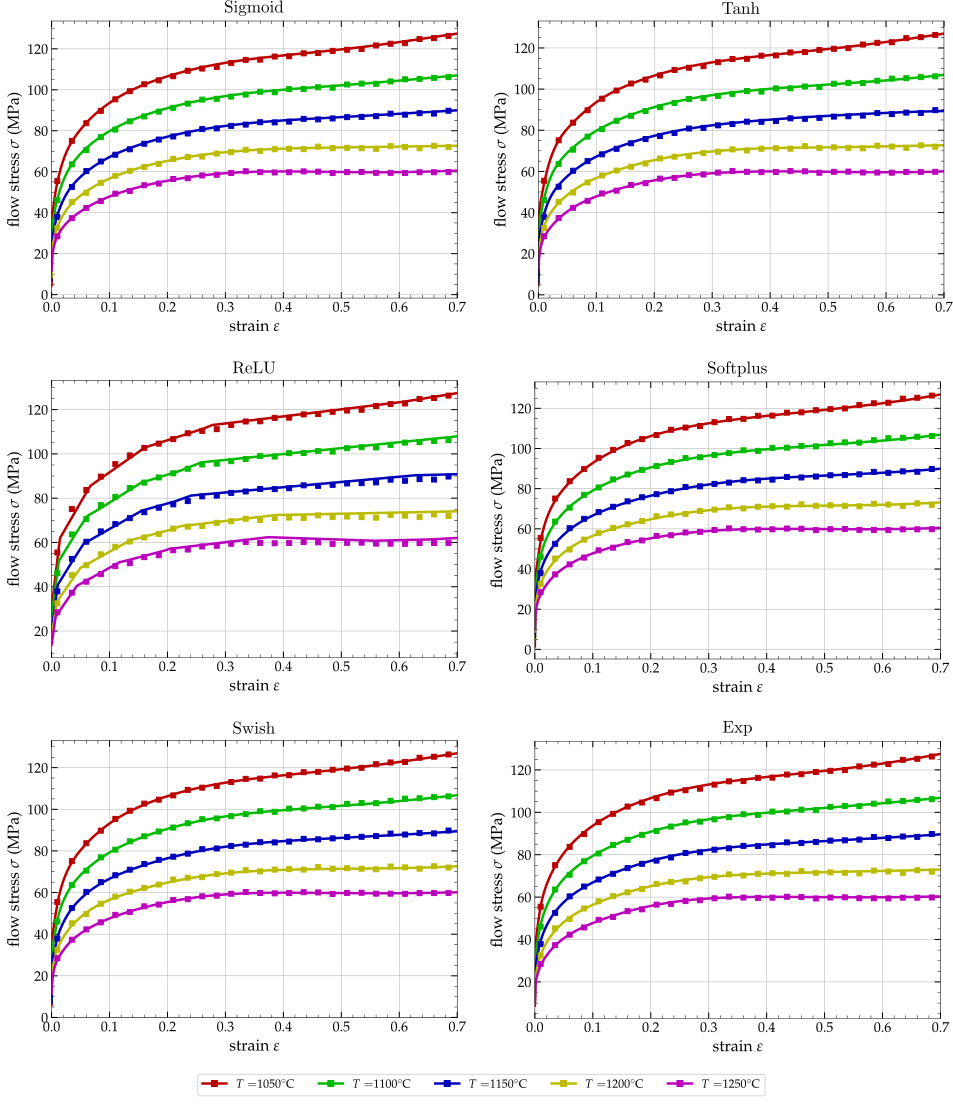
\includegraphics[width=0.95\columnwidth]{Figures/ANN-fit}
\caption{Comparison of experimental (dots) and the flow stress $\sigma$ predicted by the ANN (continuous line) for $\mdot{\varepsilon}=1~\ps$.}
\label{fig:ANNFit}
\end{figure}
From this later, we can see that all ANNs models are able to reproduce quite well the experimental results. The exception is concerning the ReLU activation function where it can be seen from the results in Figure \ref{fig:ANNFit} that the predicted flow stress enhances some piecewise linear behavior, due to its formulation and the quite low number of neurons used in the formulation of the ANN.

In this study, the error evaluation is based on the root mean square error ($\RMSE$) given by the following equation:
\begin{equation}
\RMSE (\MPa) = \sqrt{\frac{1}{N} \sum_{i=1}^{N} \left(\square_i^e - \square_i\right)^2}, \label{eq:RMSE}
\end{equation}
where $N$ is the total number of numerical training data used, $\square_i$ is the $i$th value predicted by the neural network, and~$\square_i^e$ is the corresponding experimental value coming from the experimental tests.
The accuracy and predictive ability of the models is assessed by the mean absolute relative error ($\MARE$) defined by:
\begin{equation}
\MARE(\%) = \frac{1}{N} \sum_{i=1}^{N}{\left|\frac{\square_i -\square_i^e}{\square_i^e}\right|} \times 100 \label{eq:AARE}
\end{equation}

\begin{table}[H]
\caption{Comparison of the models' error depending on the activation function used.}
\begin{tabular}{lccccc}
\toprule
Activation & Time & $\RMSE$ & $\Delta\RMSE$ & $\MARE$  & $\Delta\MARE$ \\ \midrule
ReLU & 5:14 & 1.171 & 3.422 & 4.575 & 6.350\\ 
Exp & 5:18 & 0.420 & 1.227 & 1.302 & 1.808\\ 
Sigmoid & 5:14 & 0.427 & 1.247 & 0.952 & 1.322\\ 
Tanh & 5:25 & 0.418 & 1.223 & 0.851 & 1.181\\ 
Swish & 5:31 & 0.342 & / &0.720 & / \\ 
Softplus & 5:25 & 0.394 & 1.151 & 1.070 & 1.485\\
\bottomrule
\end{tabular}
\end{table}

%\subsection{Translating of the ANN into a Fortran 77 subroutine\label{subsec:F77}}

%----------------------------------------------------------------------------------
\section{Numerical simulations using the ANN flow law}\label{sec:Numerical}
%----------------------------------------------------------------------------------

\subsection{Numerical implementation of the ANN flow law}\label{subsec:Num-impl}

\subsection{Numerical simulations and comparisons}\label{subsec:Num-sim}

The average strain rate during the compression for the center element of the specimen is around $\mdot{\overline{\varepsilon}^p}=0.8~\ps$.

\begin{table}[H]
\caption{Table}
\begin{tabular}{lcccccc}
\toprule
Activation & time & inc & inc/s & $\overline{\varepsilon}^p$ & $\overline{\sigma}$ & $T$\\ \midrule
ReLU & 915 & 1247899 & 1364 & 0.787 & 128.4 & 1071.1 \\
Exp & 998 & 1250145 & 1253 & 0.787 &122.5 &1070.5 \\
Sigmoid & 1089 & 1251869 & 1150 & 0.787 & 126.8 & 1071.1 \\
Tanh & 1202 & 1253740 & 1043 & 0.786 & 125.2 & 1070.6 \\ 
Swish & 1322 & 1246006 & 943 & 0.789 & 123.7 & 1071.0 \\
Softplus & 1795 & 1245146 & 694 & 0.783 & 125.2 & 1070.2 \\
\bottomrule
\end{tabular}
\end{table}

\begin{figure}[h]
\centering
\includegraphics[width=0.8\columnwidth]{Figures/MisesHalf}
\caption{xx.}
\label{fig:Num-misesCP}
\end{figure}

\begin{figure}[h]
\centering
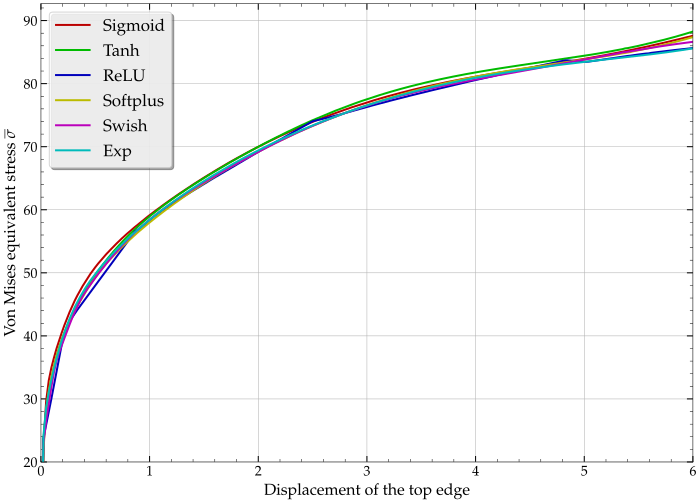
\includegraphics[width=0.8\columnwidth]{Figures/vonMises}
\caption{xx.}
\label{fig:Num-misesTH}
\end{figure}
%----------------------------------------------------------------------------------
\section{Conclusions and future work}\label{sec:Conclusions}
%----------------------------------------------------------------------------------

%%%%%%%%%%%%%%%%%%%%%%%%%%%%%%%%%%%%%%%%%%
%\section{Patents}


%%%%%%%%%%%%%%%%%%%%%%%%%%%%%%%%%%%%%%%%%%
\vspace{6pt}

%%%%%%%%%%%%%%%%%%%%%%%%%%%%%%%%%%%%%%%%%%
%% optional
%\supplementary{The following supporting information can be downloaded at:  \linksupplementary{s1}, Figure S1: title; Table S1: title; Video S1: title.}

% Only for the journal Methods and Protocols:
% If you wish to submit a video article, please do so with any other supplementary material.
% \supplementary{The following supporting information can be downloaded at: \linksupplementary{s1}, Figure S1: title; Table S1: title; Video S1: title. A supporting video article is available at doi: link.}

%%%%%%%%%%%%%%%%%%%%%%%%%%%%%%%%%%%%%%%%%%
%\authorcontributions{
%Conceptualization, P.T.M. and O.P.;
%methodology, O.P.;
%software, P.T.M. and O.P.;
%validation, O.P.;
%formal analysis, O.P.;
%investigation, P.D.;
%resources, P.D. and M.J.;
%data curation, P.T.M. and P.D.;
%writing---original draft preparation, P.T.M.;
%writing---review and editing, O.P.;
%visualization, O.P.;
%supervision, M.J., A.T. and O.P.;
%project administration, M.J.;
%funding acquisition, M.J.
%All authors have read and agreed to the published version of the manuscript.}

\funding{This research received no external funding.}

%\institutionalreview{In this section, you should add the Institutional Review Board Statement and approval number, if relevant to your study. You might choose to exclude this statement if the study did not require ethical approval. Please note that the Editorial Office might ask you for further information. Please add “The study was conducted in accordance with the Declaration of Helsinki, and approved by the Institutional Review Board (or Ethics Committee) of NAME OF INSTITUTE (protocol code XXX and date of approval).” for studies involving humans. OR “The animal study protocol was approved by the Institutional Review Board (or Ethics Committee) of NAME OF INSTITUTE (protocol code XXX and date of approval).” for studies involving animals. OR “Ethical review and approval were waived for this study due to REASON (please provide a detailed justification).” OR “Not applicable” for studies not involving humans or animals.}

%\informedconsent{Any research article describing a study involving humans should contain this statement. Please add ``Informed consent was obtained from all subjects involved in the study.'' OR ``Patient consent was waived due to REASON (please provide a detailed justification).'' OR ``Not applicable'' for studies not involving humans. You might also choose to exclude this statement if the study did not involve humans.
%
%Written informed consent for publication must be obtained from participating patients who can be identified (including by the patients themselves). Please state ``Written informed consent has been obtained from the patient(s) to publish this paper'' if applicable.}

\dataavailability{Source files of the numerical simulations are available from the author.}

%\acknowledgments{In this section you can acknowledge any support given which is not covered by the author contribution or funding sections. This may include administrative and technical support, or donations in kind (e.g., materials used for experiments).}

\conflictsofinterest{The author declare no conflict of interest.}

%%%%%%%%%%%%%%%%%%%%%%%%%%%%%%%%%%%%%%%%%%
%% Optional
%\sampleavailability{Samples of the compounds ... are available from the authors.}

%% Only for journal Encyclopedia
%\entrylink{The Link to this entry published on the encyclopedia platform.}

\abbreviations{Abbreviations}{
The following abbreviations are used in this manuscript:\\

\noindent
\begin{tabular}{@{}ll}
ANN & Artificial neural network
%AR & Arrhenius \\
%CPU & Central processing unit \\
%DRV & Dynamic recovery\\
%DRX & Dynamic recrystallization \\
%FEA & Finite element analysis \\
%HS & Hansel--Spittel \\
%JC & Johnson--Cook \\
%MZA & Modified-Zerilli--Armstrong \\
%WH & Work hardening \\
%ZA & Zerilli--Armstrong
\end{tabular}
}

%%%%%%%%%%%%%%%%%%%%%%%%%%%%%%%%%%%%%%%%%%
%% Optional
\appendixtitles{no} % Leave argument "no" if all appendix headings stay EMPTY (then no dot is printed after "Appendix A"). If the appendix sections contain a heading then change the argument to "yes".
%\appendixstart
%\appendix
%\section[\appendixname~\thesection]{}\label{sec:Appendix}

%%%%%%%%%%%%%%%%%%%%%%%%%%%%%%%%%%%%%%%%%%
\begin{adjustwidth}{-\extralength}{0cm}
%\printendnotes[custom] % Un-comment to print a list of endnotes

\reftitle{References}

% Please provide either the correct journal abbreviation (e.g. according to the “List of Title Word Abbreviations” http://www.issn.org/services/online-services/access-to-the-ltwa/) or the full name of the journal.
% Citations and References in Supplementary files are permitted provided that they also appear in the reference list here.

%=====================================
% References, variant A: external bibliography
%=====================================
\bibliography{bibliography}

% If authors have biography, please use the format below
%\section*{Short Biography of Authors}
%\bio
%{\raisebox{-0.35cm}{\includegraphics[width=3.5cm,height=5.3cm,clip,keepaspectratio]{Definitions/author1.pdf}}}
%{\textbf{Firstname Lastname} Biography of first author}
%
%\bio
%{\raisebox{-0.35cm}{\includegraphics[width=3.5cm,height=5.3cm,clip,keepaspectratio]{Definitions/author2.jpg}}}
%{\textbf{Firstname Lastname} Biography of second author}

% For the MDPI journals use author-date citation, please follow the formatting guidelines on http://www.mdpi.com/authors/references
% To cite two works by the same author: \citeauthor{ref-journal-1a} (\citeyear{ref-journal-1a}, \citeyear{ref-journal-1b}). This produces: Whittaker (1967, 1975)
% To cite two works by the same author with specific pages: \citeauthor{ref-journal-3a} (\citeyear{ref-journal-3a}, p. 328; \citeyear{ref-journal-3b}, p.475). This produces: Wong (1999, p. 328; 2000, p. 475)

%%%%%%%%%%%%%%%%%%%%%%%%%%%%%%%%%%%%%%%%%%
%% for journal Sci
%\reviewreports{\\
%Reviewer 1 comments and authors’ response\\
%Reviewer 2 comments and authors’ response\\
%Reviewer 3 comments and authors’ response
%}
%%%%%%%%%%%%%%%%%%%%%%%%%%%%%%%%%%%%%%%%%%
\PublishersNote{}
\end{adjustwidth}
\end{document}

